\subsection{Sprint 1: 19.02 \textendash 10.03.2026}\label{subsec:sprint-1}

\subsubsection{Sprint Planning 1: 19.02.2026}\label{subsubsec:sprint-planning-1}

For the planning of sprint 1 we derived all issues from the milestone project management~\ref{tab:gitlab-milestones} and had an overall weight from 89.

\subsubsection{Sprint Review 1: 10.03.2026}\label{subsubsec:sprint-review-1}

The milestone was successfully reached, and the board was cleared in preparation for the next sprint.
All issues were reviewed and moved to the \enquote{Done} column.

\paragraph{Milestone Review: Project Management}\label{par:milestone-review-project-management}

As shown in burndown and burnup charts~\ref{fig:milestone-pm-checklist-and-burndown} of the Project Planning~\ref{subsubsec:milestone-project-planning} milestone, all deliverables were fulfilled.
However, the deadlines of the milestone had to be moved to the 10.03.2026, because the project planning required more time than initially expected.
It should also be noted that the charts abruptly go down or up respectively, as we closed alot of the tickets after we reviewd them together just before we held this meeting.

\begin{figure}[H]
    \centering
    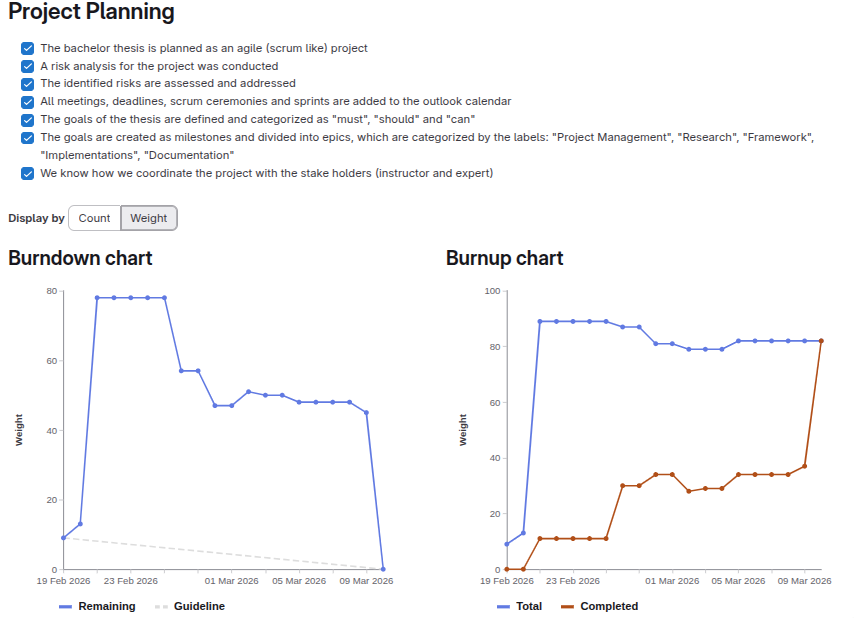
\includegraphics[width=1.0\linewidth]{../assets/screenshots/project_management/sprint_1/milestone_project_planing_charts}
    \caption{Checklist and Burndown Sprint1}
    \label{fig:milestone-pm-checklist-and-burndown}
\end{figure}

\subsubsection{Sprint Retro 1: 10.03.2026}\label{subsubsec:sprint-retro-1}

This sprint retro was held in Microsoft Whiteboard as it provides simple templates, the result is illustrated in~\ref{fig:sprint-retro-1}.

\textbf{Key Takeaways:}

\begin{itemize}
    \item Maintain clear and consistent communication with the instructor.
    \item Be aware of maintaining a healthy work\textendash{}life balance during the project.
    \item Apply lean project management practices to keep the process efficient and focused.
\end{itemize}

\begin{figure}[H]
    \centering
    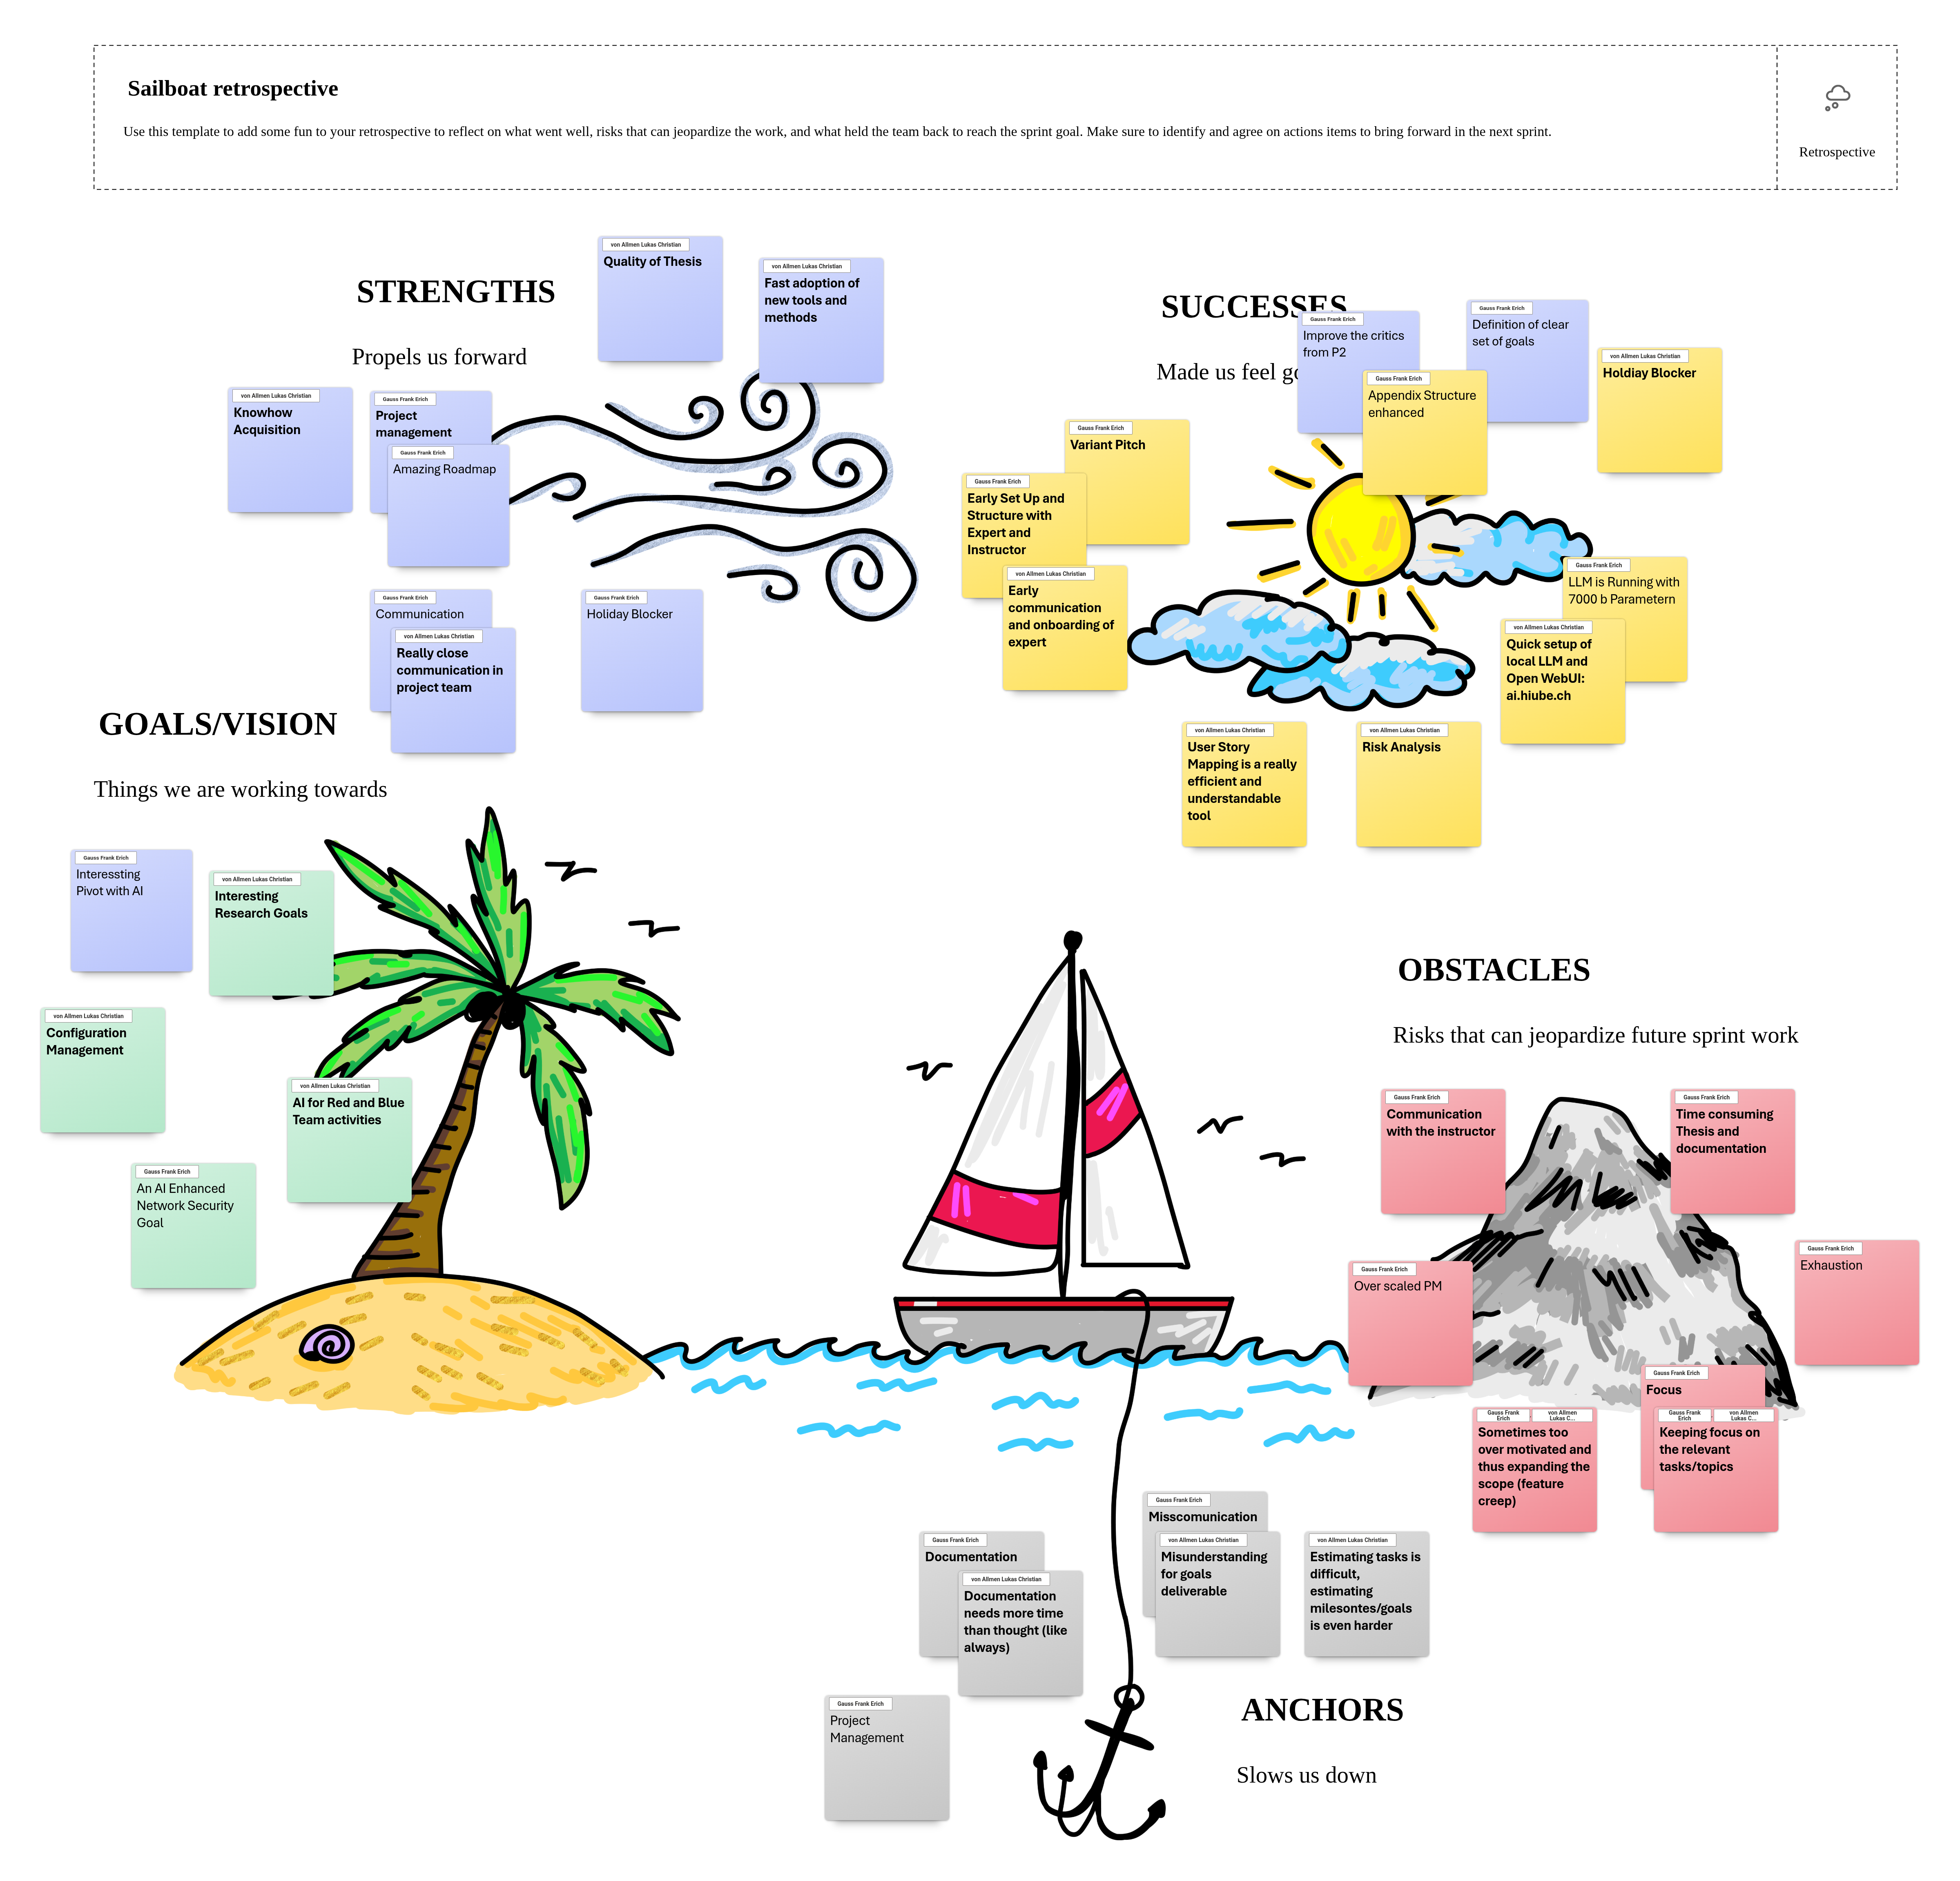
\includegraphics[width=1.0\linewidth]{../assets/screenshots/project_management/sprint_1/sprint_retro_1}
    \caption{Sprint Retro 1}
    \label{fig:sprint-retro-1}
\end{figure}
